%!TEX root = ../thesis.tex
%*******************************************************************************
%****************************** Fourth Chapter *********************************
%*******************************************************************************

\chapter{Benchmark}
\label{chap:benchmark}
\ifpdf
    \graphicspath{{Chapter4/Figs/Raster/}{Chapter4/Figs/PDF/}{Chapter4/Figs/}}
\else
    \graphicspath{{Chapter4/Figs/Vector/}{Chapter4/Figs/}}
\fi

\section{Constitution du benchmark} % (fold)
\label{sec:constitution_du_benchmark}


\section{Data} % (fold)
\label{sec:data}

\subsection{Apple and pears} % (fold)
\label{sub:apple_and_pears}

Let's start with a toy problem and make it gradually more complex.
The study is about finding the proportion $\mu$ of apples and pears in a bag.
The only information available is the total number of fruits in the bag and the weight of each individual fruit.
Apples and pears weights are normally distributed and slightly different.
The dataset is a set of real values $D = \{ x_i \in \RR \} $

From the average weight of the fruits in the bag a linear regression is enough to find the link between $D$ and the parameter of interest $\mu$.
The model can be trained if enough bags in which the proportion is known is available for training.
This simplicity is wanted to test the method.

Since the weight of a fruit is stochastic, two bags of fruits with the same number of apples and pears may have a different average weight.
Leading to some uncertainty in the predicted proportion that must be reported.

\subsection{Toy 1D} % (fold)
\label{sub:toy_1d}


\subsection{Toy 3D} % (fold)
\label{sub:toy_3d}


L'exemple jouet introduit dans \cite{DECASTRO2019170inferno} est un mélange de 2 processus (background \& signal)


Pour les backgrounds :
$$
f_b (x|r, \lambda) = \mathcal N \left ( (x_0, x_1) | (2+r, 0) 
\begin{bmatrix} 5 & 0 \\ 0 & 9 \end{bmatrix} \right ) Exp((x_2| \lambda)
$$


Pour les signaux :
$$
f_s (x|r, \lambda) = \mathcal N \left ( (x_0, x_1) | (1, 1) 
\begin{bmatrix} 1 & 0 \\ 0 & 1 \end{bmatrix} \right ) Exp((x_2| 2)
$$

Ce qui donne la vraissemblance :
$$
p(x | r, \lambda, \mu ) = (1-\mu) f_b(x|r, \lambda) + \mu f_s(x|r, \lambda)
$$

Ce toy a l'avantage d'être multidimensionnel et plus complexe que le précédent.


\begin{figure}[htb]
    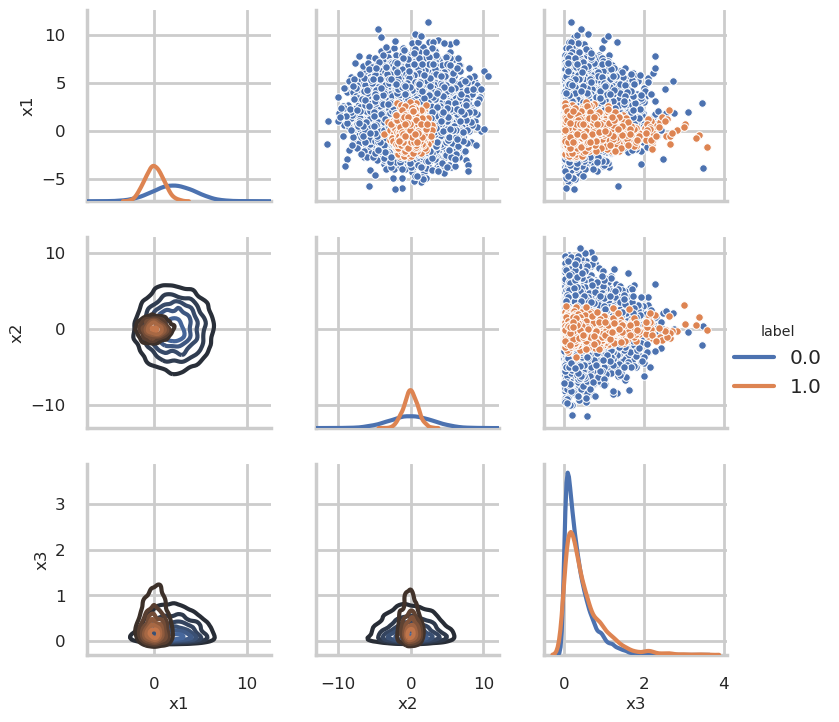
\includegraphics[width=\linewidth]{s3d2/pairgrid}
    \caption{Data distribution of the 3D toy}
    \label{fig:s3d2_pairgrid}
\end{figure}


\subsection{Higgs data} % (fold)
\label{sub:higgs_data}

\content{importance weight}
\content{nuisance parameters}
\content{simulateur rapide}




\section{Evaluation metric} % (fold)
\label{sec:evaluation_metric}

\topic{The evaluation metric is the empirical mean squared error on the estimated parameters including variances}

Many methods to estimate the parameter of interest and its variance are available.
If changing the set of hyper parameter for the learning procedure is considered as changing the method then countless methods are to be evaluated.
Automating the measure of the performances of a proposed method is crucial to select the best method.
In this section is described a simple but general procedure to measure the performances of a given method.

The usual criterions to evaluate an estimator $\htheta$ are the bias, the variance and the mean squared error defined as follow :
\begin{equation}
  Bias(\htheta) = \EE[\htheta] - \thetas
\end{equation}
\begin{equation}
  Var(\htheta) = \EE[ (\htheta - \EE[\htheta])^2 ] = \EE[\htheta^2] - (\EE[\htheta])^2
\end{equation}
\begin{equation}
  MSE(\htheta) = \EE[(\htheta - \thetas)^2] = Var(\htheta) + [Bias(\htheta)]^2
\end{equation}

To evaluate these criterion we need to repeat the experiement $N$ times leading to many estimation of the parameters $\hmu^{(k)}$ and $\hshmu^{(k)}$.
Repeating the experiment can be done through cross-validation methods.


\subsection{Evaluation of the parameter of interest estimator} % (fold)
\label{sub:evaluation_of_the_parameter_of_interest_estimator}

First, let's focus on evaluating the estimator of the parameter of insterest $\hmu$.
The true value of $\mu$, noted $\mus$, is available during tests since it is an input of the simulator.

From the estimation of its expected value
\begin{equation}
  \EE[\hmu] \approx <\hmu^{(k)}>_k = \frac{1}{N} \sum_{k} \hmu^{(k)}
\end{equation}
it is possible to estimated the criterions

\begin{equation}
  Bias(\hmu) \approx <\hmu^{(k)}>_k - \mus
\end{equation}
\begin{equation}
  \label{eq:var_hmu}
  Var(\hmu) \approx <\hmu^{(k)} \times \hmu^{(k)}>_k - (<\hmu^{(k)}>_k)^2
\end{equation}
\begin{equation}
  MSE(\hmu) = Var(\hmu) + [Bias(\hmu)]^2
\end{equation}

\subsection{Evaluation of the variance estimator} % (fold)
\label{sub:evaluation_of_the_variance_estimator}

The evaluation of the variance estimator $\hshmu$ could be done in the same way if the true variance $Var(\hmu)$ can be computed.
If this is not the case an approximation is available using \autoref{eq:var_hmu}.

\begin{equation}
  Bias(\hshmu) \approx <\hshmu^{(k)}>_k - Var(\hmu)
\end{equation}
\begin{equation}
  Var(\hshmu) \approx <\hshmu^{(k)} \times \hshmu^{(k)}>_k - (<\hshmu^{(k)}>_k)^2
\end{equation}
\begin{equation}
  MSE(\hshmu) = Var(\hshmu) + [Bias(\hshmu)]^2
\end{equation}




